\documentclass{article}
\usepackage[utf8]{inputenc}
\usepackage{graphicx}
\usepackage{amsmath}
\usepackage{amssymb}
\usepackage[utf8]{inputenc}
\usepackage[english]{babel}
\usepackage{amsthm}
\usepackage{makecell,tabularx}
\usepackage{hyperref}

\newtheorem{theorem}{Theorem}[section]
\newtheorem{corollary}{Corollary}[theorem]
\newtheorem{lemma}[theorem]{Lemma}
\theoremstyle{definition}
\newtheorem{definition}{Definition}[section]

\hypersetup{colorlinks,urlcolor=blue}
%% or
% \hypersetup{colorlinks=false,pdfborder=000}

% hack into hyperref
\makeatletter
\DeclareUrlCommand\ULurl@@{%
  \def\UrlFont{\ttfamily\color{blue}}%
  \def\UrlLeft{\uline\bgroup}%
  \def\UrlRight{\egroup}}
\def\ULurl@#1{\hyper@linkurl{\ULurl@@{#1}}{#1}}
\DeclareRobustCommand*\ULurl{\hyper@normalise\ULurl@}
\makeatother

\graphicspath{ {images/} }

\title{Coursera Notes}
\author{Siavash Aslanbeigi}
\date{April 2018}

\begin{document}

\maketitle
\tableofcontents

% INTRODUCTION =========================================
\section{Introduction}
Machine learning is a collection of techniques which allow computers to complete tasks by learning from data. It grew out of work in Artificial Intelligence (AI). Traditionally, we program computers to do what we want by giving them precise instructions. There are problems for which this technique doesn't work very well. 

Consider the problem of recognizing hand-written digits: given an image of a hand-written digit, the computer is supposed to map it to the corresponding digit, i.e. pick correctly from $0,1,\dots,9$. Figure \ref{intro-fig:mnist-examples} shows examples of hand-written digits. It is quite easy for a human to recognize these digits correctly, even though none of them have the exact same shape. Programming a computer to do the same turns out to be very difficult. The reason is that it's impossible to explicitly tell the computer about all possible shapes; there are just too many of them. Machine learning approaches this problem differently: we present the algorithm images like those shown in Figure \ref{intro-fig:mnist-examples} (input), as well as the correct digits they represent (output), and let the algorithm figure out for itself what the correct way of recognizing hand-written digits is. Once the algorithm is trained on the data, we can use it to recognize digits not in the dataset, i.e. to make predictions. This technique has proved more reliable than any other approach so far. It also seems more inline with how humans learn from experience.

\begin{figure}[ht]
\centering
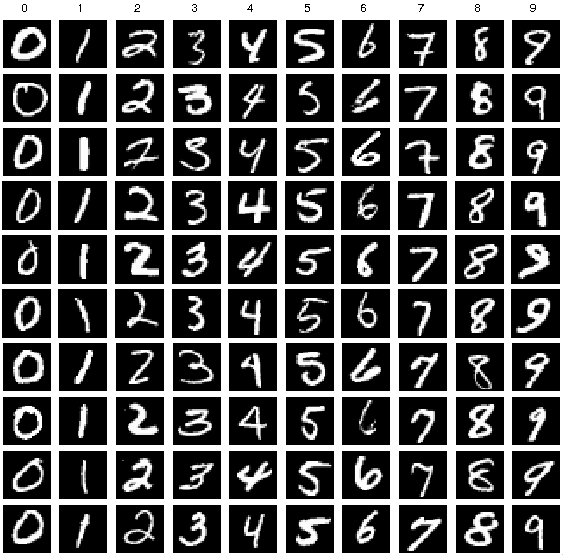
\includegraphics[scale=0.4]{images/intro/mnist-ex.png}
\caption{Examples of handwritten digits from the MNIST dataset.}
\label{intro-fig:mnist-examples}
\end{figure}
Other modern applications of machine learning include:
\begin{itemize}
    \item Spam filters: it is impossible to explicitly list all possible spam emails one might receive.
    \item Database mining: growth of automation/web has resulted in much larger data sets which need to be understood. Examples include web click data, medical records, etc.
    \item Natural Language Processing (NLP), whose aim is to make computers understand text.
    \item Self-customizing programs, such as Netflix product recommendations.
    \item Understanding the human brain. How is it that we humans learn?
\end{itemize}
Here are two formal definitions of machine learning:
\begin{itemize}
    \item Arthur Samuel (1959): Field of study that gives computers the ability to learn without being explicitly programmed. Samuel built a Checkers playing program where the computer would learn from playing tens of thousands of games against itself. This was the world's first self-learning program.
    \item Tom Mitchell (1998): A computer program is said to learn from experience E with respect to some task T and some performance measure P, if its performance on T, as measured by P, improves with experience E.
\end{itemize}
There are two main types of machine learning algorithms: supervised-learning and unsupervised learning.

% Supervised learning ----------------------------------
\subsection{Supervised learning}
Supervised learning is the most common type of machine learning problem. The name \textbf{supervised} comes from the fact that the training samples (i.e. our data) contain the "right answers". In other words, for a set of inputs, we know what the output should be. Suppose we have the following data for prices of houses:

\begin{figure}[ht]
\centering
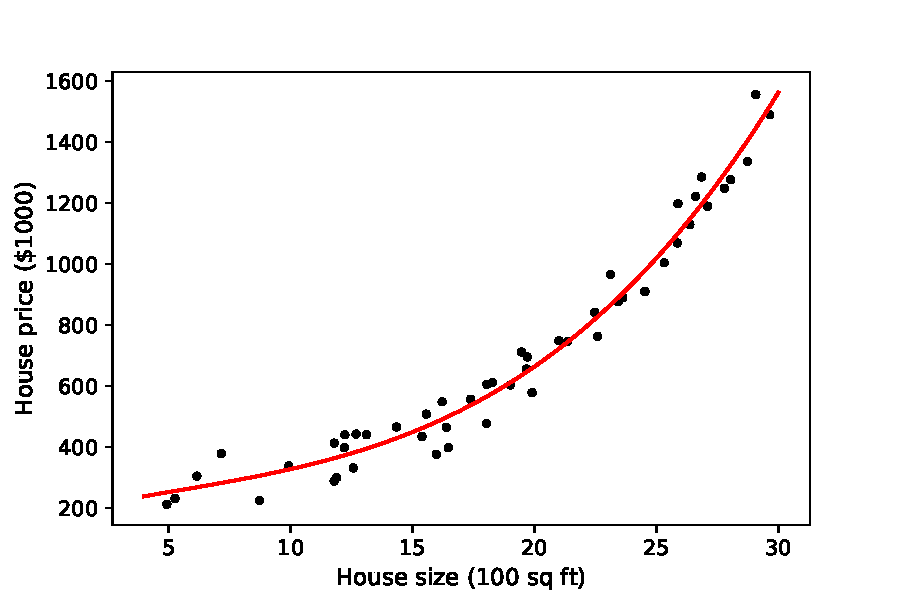
\includegraphics[scale=0.7]{images/lin_reg/poly-data.pdf}
\caption{Predicting house prices.}
\label{into-house-prices}
\end{figure}

What is the price of a house which is $800 \text{ft}^2$? Although none of the houses in our data set have that size, we could make a prediction by fitting a curve through the data points, as shows in Figure \ref{into-house-prices}.

Supervised learning algorithms fall in two broad categories:
\begin{itemize}
    \item \textbf{Regression}: output values are continuous, for instance, predicting house prices, stock prices, etc.
    \item \textbf{Classification}: output values are discrete, for instance whether or not a tumor is malignant or benign.
\end{itemize}

Suppose we have a data set about breast tumors: we are given the size of each tumor, age of the patient, and whether or not it's malignant.

\begin{figure}[ht]
\centering
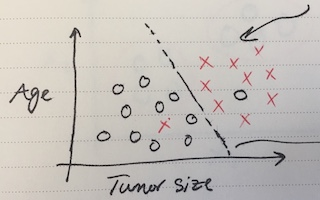
\includegraphics[scale=0.8]{images/intro/tumor.jpg}
\caption{Predicting whether new tumor is malignant or benign. Circles denote benign tumors, and Xs malignant ones.}
\label{intro-tumor}
\end{figure}

Given a new tumor, we'd like to be able to predict whether or not it's malignant or benign. This is an example of a classification problem, since the output values are discrete (we can assign $0$ to benign tumors, and $1$ to malignant ones.) The learning algorithm may decide that the line drawn in Figure \ref{intro-tumor} separates benign and malignant tumors.

% Unsupervised learning --------------------------------
\subsection{Unsupervised learning}
In supervised learning, the training samples tell us the correct outputs for a set of inputs. We then seeks to predict the output for new examples. Unsupervised learning is different in that we not given the right answers. It's more like, here's a data set, find some structure in it. For instance, a learning algorithm may tell us that in Figure \ref{intro-clustering} most of the data is concentrated in two different regions,those which are circled. This is an example of a clustering algorithm.

\begin{figure}[ht]
\centering
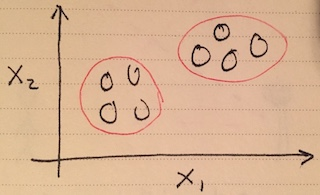
\includegraphics[scale=0.8]{images/intro/clustering.jpg}
\caption{Clustering algorithm.}
\label{intro-clustering}
\end{figure}

A real-life application of clustering is Google News, which looks at thousands of news and groups similar ones together. For instance, it would recognize that these articles from different sources are about the same topic and clusters them together:

\begin{itemize}
    \item The Source: BP kills Macondo, but its legacy lives on.
    \item CNN: Well is dead, but much Gulf Coast work remains.
    \item Guardian: BP oil spill costs nearly $\$10$bn dollars.
\end{itemize}

How remarkable is this? Here's another example of an unsupervised learning algorithm: the cocktail party problem, demonstrated in Figure \ref{intro-cocktail}.

\begin{figure}[ht]
\centering
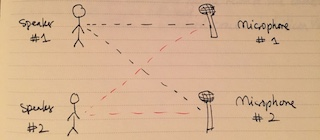
\includegraphics[scale=0.8]{images/intro/cocktail.jpg}
\caption{Cocktail party problem.}
\label{intro-cocktail}
\end{figure}

Two people are talking at the same time. In microphone 1, the sound of speaker 1 is recorded more loudly than speaker 2, simply because speaker 1 is closer to microphone 1, and vice versa for microphone 2. If the volume offsets are pronounced enough, a human would easily recognize by listening to the recording of microphones 1 and 2 that there are two speakers, and even what each of them is saying. The amazing thing is that there are unsupervised learning algorithms that are capable of doing the same. Based on the volume offsets, they recognize the structures of the two speakers sounds and are able to separate them out.


% Linear regression with one variable ==================
\section{Linear regression with one variable}
Consider a \textit{training set} (data set which we'll use to fit parameters of our model, or \textit{train} our model) for house prices in Portland, OR:

\begin{center}
\begin{tabular}{ |c|c| } 
 \hline
 Size ($\text{ft}^2$) (x) & Price ($\$1000$) (y) \\
 \hline
 2104 & 460 \\
 1416 & 232 \\
 1534 & 315 \\
 852 & 178 \\
 \vdots & \vdots \\
 \hline
\end{tabular}
\end{center}

Our job is to learn from this data how to predict prices of houses as a function of their size. This is a supervised learning problem, because our training set contains the right answers: for every input (house size), we know the right output (house price). Moreover, this is a regression problem, because the output variable (house price) is continuous. Figure \ref{linreg-bigpic} shows the picture of how we will tackle this problem: given the training set, our learning algorithm will spits out a function $h$, called the \textit{hypothesis} function, which can estimate the price of a house given its size.

\begin{figure}[ht]
\centering
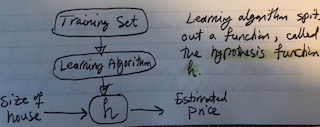
\includegraphics[scale=0.8]{images/lin_reg/big-picture.jpg}
\caption{Big picture.}
\label{linreg-bigpic}
\end{figure}

% Model representation ---------------------------------
\subsection{Model representation}
How do we represent $h$? We start with the simplest function possible and consider more complex models later:
\begin{equation}
    h_{\theta}(x) = \theta_0 + \theta_1 x.
    \label{linreg-eq:univar-hypothesis}
\end{equation}
This function assumes a linear relationship between the size of a house $x$ and its price $h_{\theta}(x)$. It is sometimes referred to as \textit{univariate linear regression}, because it is a function of a single variable (size of house) and is linear. We will come up with a learning algorithm that uses the training set to estimate the coefficients $\theta_0$ and $\theta_1$. With that at our disposal, we can predict the price of a house given its size. 

% Cost function ----------------------------------------
\subsection{Cost function}
What values of $\theta_0$ and $\theta_1$ provide the best "fit" to our training? Let's start by establishing notation:
\begin{itemize}
    \item $m$: Number of training examples.
    \item $x$: Input variable/feature (size of house).
    \item $y$: Output variable/target variable (price of house).
    \item $(x^{(i)}, y^{(i)})$: $i^{\text{th}}$ training example (size and price of a house in our training set).
\end{itemize}

For a given house size $x^{(i)}$ in our training set, we know the correct house price $y^{(i)}$. It then makes sense to pick $\theta_0$ and $\theta_1$ so that $h_{\theta}(x^{(i)})$ is as close to $y^{(i)}$ as possible. Realistically, we cannot tune $\theta_0$ and $\theta_1$ so that $h_{\theta}(x^{(i)})=y^{(i)}$ for all examples, since we only have two parameters to play with but many more examples ($m \gg 2$) to fit. As a result, we need to strike a balance across all examples, so that the collective prediction error $|h_{\theta}(x) - y|$ on the training set is minimized. To that end, consider the following function, called the \textit{cost function}:

\begin{align}
    J(\theta_0, \theta_1) &= \frac{1}{2m}\sum_{i=1}^{m}(h_{\theta}(x^{(i)}) - y^{(i)})^2
    \label{linreg-eq:costfunc}\\
    &= \frac{1}{2m}\sum_{i=1}^{m}(\theta_0 + \theta_1 x^{(i)} - y^{(i)})^2
    \label{linreg-eq:univar-costfunc}
\end{align}
Given $\theta_0$ and $\theta_1$, it computes the sum of (squared) prediction errors across all training examples. (It also normalizes the sum by $2m$, but that's only for mathematical convenience.) We can think about $J$ as measuring the \textit{cost} of the model's predicted house prices deviating from actual house prices in the training set. So, it makes sense to pick the values of $\theta_0$ and $\theta_1$ that minimize $J$. Figure \ref{linreg-fig:costfunc} shows the correspondence between minimizing $J$ and getting a better fit to to the training set. 

\begin{figure}[ht]
\centering
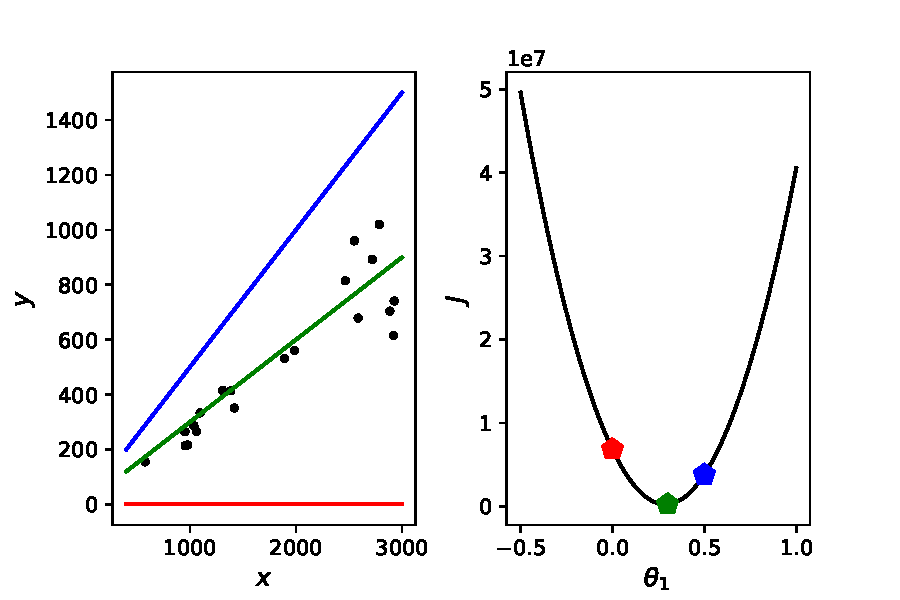
\includegraphics[scale=0.7]{images/lin_reg/costfunc.pdf}
\caption{Correspondence between minimizing the cost function and getting a better fit to data. The following model is used to fit the data: $h_{\theta}(x) = \theta_1 x$. Black dots on the left show the training set. The right figure shows the cost function $J(\theta_1)$. Every dot on the right figure corresponds to a line of the same color on the left figure. We see that the closer $\theta_1$ is to $J$'s minimum, the better the fit to data is. Code used to generate this plot can be found \href{https://github.com/siavashaslanbeigi/ml_notes_supp/blob/master/lin_reg/costfunction.ipynb}{here}.}
\label{linreg-fig:costfunc}
\end{figure}

Why cost function \eqref{linreg-eq:univar-costfunc} and not some other one? There are plenty of other cost functions whose minimization would also lead to a good fit of data. For linear regression, though, \eqref{linreg-eq:univar-costfunc} does have some desirable mathematical properties. First of all, $J$ is a quadratic function of $\theta_0$ and $\theta_1$, i.e. it's a paraboloid. As a result, it doesn't have any local minima, only a global one. This makes minimization a much easier task. Secondly, as we will show in the next section, minimization of $J$ can be carried out analytically.

% Minimizing the cost function -------------------------
\subsection{Minimizing the cost function}
The global minimum of $J$ occurs where its gradient is zero:
\begin{align*}
    \frac{\partial J}{\partial\theta_0} &= \frac{1}{m}\sum_{i=1}^{m}(\theta_0 + \theta_1 x^{(i)} - y^{(i)}) = 0 \\
    \frac{\partial J}{\partial\theta_1} &= \frac{1}{m}\sum_{i=1}^{m}(\theta_0 + \theta_1 x^{(i)} - y^{(i)})x^{(i)} = 0.
\end{align*}
Thus, we have to solve the following system of linear equations
\begin{align*}
    m \theta_0 + \left[\sum_{i=1}^{m}x^{(i)}\right]\theta_1 &= \sum_{i=1}^{m} y^{(i)}\\
    \left[\sum_{i=1}^{m}x^{(i)}\right] \theta_0 + \left[\sum_{i=1}^{m}\left(x^{(i)}\right)^2\right]\theta_1 &= \sum_{i=1}^{m} x^{(i)}y^{(i)},
\end{align*}
the solution to which is given by
\begin{equation}
\begin{pmatrix}
\theta_0\\
\theta_1
\end{pmatrix}
=
\begin{pmatrix}
m & \sum_{i=1}^{m}x^{(i)}\\
\sum_{i=1}^{m}x^{(i)} & \sum_{i=1}^{m}\left(x^{(i)}\right)^2
\end{pmatrix}^{-1}
\begin{pmatrix}
\sum_{i=1}^{m}y^{(i)}\\
\sum_{i=1}^{m}x^{(i)}y^{(i)}
\end{pmatrix}.
\label{linreg-eq:univar-sol}
\end{equation}
We have solved the problem we posed in the beginning of this section. Given the training set, we can use \eqref{linreg-eq:univar-sol} to estimate $\theta_1$ and $\theta_2$, and then make predictions using \eqref{linreg-eq:univar-hypothesis}.


% Linear regression with multiple variables ============
\section{Linear regression with multiple variables}
In the previous section, we wanted to predict the price of a house as a function of its size. Of course, there are many more factors would could affect house prices:

\begin{center}
\begin{tabularx}{\linewidth}{ |l|X|X|X|l| } 
 \hline
 \thead{Size (ft$^2$) ($x_1$)} &
 \thead{Number of\\ bedrooms ($x_2$)} &
 \thead{Number of\\ floors ($x_3$)} &
 \thead{Age of home\\ (years) ($x_4$)} &
 \thead{Price (\$1000) (y)}\\
 \hline
 2104 & 5 & 1 & 45 & 460 \\
 1416 & 3 & 2 & 40 & 232 \\
 1534 & 3 & 2 & 30 & 315 \\
 852 & 2 & 1 & 10 & 178 \\
 \vdots & \vdots & \vdots & \vdots & \vdots\\
 \hline
\end{tabularx}
\label{linreg-tab:houseprice}
\end{center}

The independent variables $x_1-x_4$ (e.g. size of house, number of bedrooms, etc), which we think the output variable depends on, are called \textit{features}. In this section, we will generalize the univariate linear regression to incorporate more than just one feature.


% Model representation ---------------------------------
\subsection{Model representation}
We start by establishing notation:

\begin{itemize}
    \item $n$: Number of features.
    \item $x^{(i)}_{j}$: Value of $j$th feature in the $i$th training example.
\end{itemize}
For data shows in Table \ref{linreg-tab:houseprice}: $n=4$, $x^{(2)}_3=2$, etc. We generalize the univariate hypothesis \eqref{linreg-eq:univar-hypothesis} to a multivariate one as follows:
\begin{equation}
    h_{\theta}(x) = \theta_0 + \theta_1x_1 + \theta_2x_2 + \cdots + \theta_nx_n.
    \label{linreg-eq:multi-hypothesis}
\end{equation}
Let's establish more notation, so we can write \eqref{linreg-eq:multi-hypothesis} in matrix form:
\begin{itemize}
    \item $x_0 \equiv 1$. In other words, $x^{(i)}_0 = 1$ for all $i$.

    \item $x=
        \begin{pmatrix}
            x_0 \\
            x_1 \\
            \vdots \\
            x_n
        \end{pmatrix}
        \in \mathbb{R}^{n+1}
    $ denotes the vector of features.

    \item $x^{(i)}=
        \begin{pmatrix}
            x^{(i)}_0 \\
            x^{(i)}_1 \\
            \vdots \\
            x^{(i)}_n
        \end{pmatrix}
        \in \mathbb{R}^{n+1}
    $ denotes the vector of features for the $i$th training example. 

    \item $\theta =
        \begin{pmatrix}
            \theta_0 \\
            \theta_1 \\ 
            \vdots \\
            \theta_n
        \end{pmatrix}
        \in \mathbb{R}^{n+1}
    $ is the vector of parameters.
\end{itemize}
We have created a fictitious feature $x_0$ whose value is always set to $1$. This helps us rewrite the hypothesis function in matrix form:
\begin{equation}
    h_{\theta}(x) = \theta^Tx.
    \label{linreg-eq:multi-hypothesis-mat}
\end{equation}


% Cost function ----------------------------------------
\subsection{Cost function}
We will use the same cost function \eqref{linreg-eq:costfunc}, but with hypothesis \eqref{linreg-eq:multi-hypothesis}:
\begin{align}
    J(\theta) &= \frac{1}{2m}\sum_{i=1}^{m}(h_{\theta}(x^{(i)}) - y^{(i)})^2 \notag\\
    &= \frac{1}{2m}\sum_{i=1}^{m}(\theta^Tx^{(i)} - y^{(i)})^2.
    \label{linreg-eq:multi-costfunc}
\end{align}
Now $J$ is a function of $n+1$ variables ($\theta_0, \theta_1, \dots, \theta_n$), and we will need to find the vector $\theta$ that minimizes $J$. Before dealing with the minimization problem, let's rewrite $J$ in a more compact form. Consider the following definitions:
\begin{itemize}
    \item Design matrix $X$: $m \times (n+1)$ matrix whose elements are given by $X_{ij} = x^{(i)}_j$. Every row corresponds to a training example, and every column to a feature.
    \item Target vector $Y$: $m$-dimensional vector of all outputs in the training set, i.e. $Y_i=y^{(i)}$.
\end{itemize}
For data shows in Table \ref{linreg-tab:houseprice}, the design matrix and target vector are given by
\begin{equation}
    X =
    \begin{pmatrix}
        1 & 2104 & 5 & 1 & 45 \\
        1 & 1416 & 3 & 2 & 40 \\
        1 & 1534 & 3 & 2 & 30 \\
        1 & 852 & 2 & 1 & 10 \\
        \vdots & \vdots & \vdots & \vdots & \vdots \\
    \end{pmatrix},
    \qquad
    Y =
    \begin{pmatrix}
        460 \\
        232 \\
        315 \\
        178 \\
        \vdots
    \end{pmatrix}.
\end{equation}
With these definitions, we can show that $\theta^Tx^{(i)}$ is the $i$th component of the the $m$-dimensional vector $X\theta$: $\theta^Tx^{(i)}=\sum_{j=0}^n\theta_jx^{(i)}_j=\sum_{j=0}^nX_{ij}\theta_j=[X\theta]_i$. This in turn helps us write $J$ in terms of the squared norm of the vector $X\theta - Y$:
\begin{align}
    J(\theta) &= \frac{1}{2m}\sum_{i=1}^{m}(\theta^Tx^{(i)} - y^{(i)})^2\notag\\
    &= \frac{1}{2m}\sum_{i=1}^{m}([X\theta]_i - Y_i)^2\notag\\
    &= \frac{1}{2m}\sum_{i=1}^{m}[X\theta - Y]_i[X\theta - Y]_i\notag\\
    &= \frac{1}{2m}(X\theta - Y)^T(X\theta - Y).
    \label{linreg-eq:multi-costfunc-mat}
\end{align}

Why do we care to write $J$ in matrix (or sometimes called \textit{vectorized}) form? One reason is parallelization: matrix multiplication is a highly parallelizable operation. Consider $C=AB$, where $A$ and $B$ are $1000,000 \times 5$ and $5 \times 1$ dimensional, respectively. All $1000,000$ components of $C$ can be computed in parallel, because they do not depend on one another. Most programming languages have highly optimized libraries for matrix multiplication. In the following Python \href{https://github.com/siavashaslanbeigi/machine_learning/blob/master/lin_reg/matrix.ipynb}{\color{blue} example}, it's shown that a vectorized implementation of \eqref{linreg-eq:multi-costfunc-mat} is more than two orders of magnitude faster than a for-loop implementation of \eqref{linreg-eq:multi-costfunc}. This is not all due to parallelization; overhead of the for-loops itself is probably a major factor. This should, however, serve to demonstrate the importance of vectorized implementations for large data sets.

Writing expressions in matrix form also makes it easier to see when linear algebra results could be relevant. For instance, later in this section we will use the eigen-values and eigen-vectors of $X^TX$ to show that minimization of $J$ does not lead to a unique solution for $\theta$ when $m<n+1$.


% Normal equation --------------------------------------
\subsection{Normal equation}
Just like the univariate case, $J$ is a quadratic function of $\theta_0, \theta_1, \dots, \theta_n$, and its global minimum occurs where its gradient is zero. Let's compute the gradient of $J$ with respect to $\theta_j$:
\begin{align*}
    \frac{\partial J}{\partial \theta_j} &= \frac{1}{m}\sum_{i=1}^{m}(\theta^Tx^{(i)} - y^{(i)})x^{(i)}_j\\
    &=\frac{1}{m}\sum_{i=1}^{m}[X\theta - Y]_iX_{ij}\\
    &=\frac{1}{m}[X^T(X\theta - Y)]_j,
\end{align*}
or equivalently
\begin{equation}
    \nabla_{\theta} J = \frac{1}{m}X^T(X\theta - Y).
\end{equation}
As a sanity check, note that the dimensions of the two sides match: $\nabla_{\theta} J$ is an ($n+1$)-dimensional vector, and $X^T(X\theta - Y)$ is a multiplication between a $(n+1) \times m$ and $m \times 1$ matrix, which again is an ($n+1$)-dimensional vector. Setting the gradient to zero, we arrive at the value of $\theta$ that minimizes:
\begin{equation}
    \theta = \left(X^TX\right)^{-1}X^TY.
    \label{linreg-eq:normal}
\end{equation}
This is called the \textit{normal} equation. You should check for yourself that \eqref{linreg-eq:normal} reduces to \eqref{linreg-eq:univar-sol} when $n = 1$.

So there we have it. Given the training set in the form of the design matrix $X$ and the target vector $Y$, we can estimate $\theta$ via \eqref{linreg-eq:normal} and then use \eqref{linreg-eq:multi-hypothesis-mat} to make predictions for new examples.


% When the normal equation fails -----------------------
\subsection{When the normal equation fails}
The normal equation \eqref{linreg-eq:normal} can only work if $X^TX$ is invertible. Let's look at scenarios where this is not the case, and understand the reasons intuitively and mathematically. Consider the following design matrix, constructed using the first two examples in table \ref{linreg-tab:houseprice}:
\begin{equation}
    X =
    \begin{pmatrix}
        1 & 2104 & 5 & 1 & 45 \\
        1 & 1416 & 3 & 2 & 40 \\
    \end{pmatrix}.
    \label{linreg-eq:design-mat-noninvert}
\end{equation}
It can be checked that $\text{det}(X^TX)=0$. Therefore, $X^TX$ is not invertible. Is there something special about this data set? As it turns out, this result holds no matter how we tweak the numbers. This may seem a bit surprising. However, let's consider what it would've meant if $X^TX$ was invertible. The dataset contains five features (including $x_0$), so the normal equation will solve for five parameters $\theta_0,\theta_1\dots\theta_4$, but using only two examples. In short, there are two equations and five unknowns. There's not enough data to fix the parameters of the model, which manifests itself through the non-invertibility of $X^TX$.

More generally, we should expect that $X^TX$ is not invertible when $m<n+1$, i.e. when there are fewer examples than features.
Let's prove this. We will make use of the Singular Value Decomposition (SVD), which states that any matrix $m\times n$ can be written as
\begin{equation}
    A = UDV^T,
\end{equation}
where:
\begin{itemize}
    \item $U$ is an $m\times m$ matrix which satisfies $U^TU=UU^T=1_m$, where $1_m$ is the $m$-dimensional identity matrix.
    \item $V$ is an $n\times n$ matrix which satisfies $V^TV=VV^T=1_n$, where $1_n$ is the $n$-dimensional identity matrix.
    \item $D$ is an $m\times n$ matrix with zero elements everywhere except $D_{ii}\ge0$ where $i=1,\dots,\text{min}(m, n)$. So $D$ is diagonal and has at most $\text{min}(m, n)$ elements on the diagonal. These elements are called the singular values of $X$.
\end{itemize}
It can be checked that \eqref{linreg-eq:design-mat-noninvert} admits the following SVD:
\begin{align*}
    U &=
    \begin{pmatrix}
        -1 & 1 \\
        -1 & 1 \\
    \end{pmatrix} \\
    D &= 
    \begin{pmatrix}
        2537 & 0 & 0 & 0 & 0 \\
        0 & 8 & 0 & 0 & 0 \\
    \end{pmatrix} \\
    V &= 
    \begin{pmatrix}
        0 & 0 & 0 & 0 & -1 \\
        -1 & 0 & 0 & 0 & 0 \\
        0 & 0 & 1 & 0 & 0 \\
        0 & 0 & 0 & 1 & 0 \\
        0 & 1 & 0 & 0 & 0 \\
    \end{pmatrix}. 
\end{align*}
We can now express $X^TX$ in terms of the SVD of the design matrix $X=UDV^T$ (remember that $X$ is $m\times (n+1)$ dimensional, so $D$ and $V$ are $m\times (n+1)$ and $(n+1)\times (n+1)$ dimensional, respectively):
\begin{align*}
    X^TX &= (UDV^T)^T(UDV^T)\\
    &= VD^TU^TUDV^T \\
    &=VD^TDV^T,
\end{align*}
where in the third equality we've used $U^TU=1_m$. Taking the determinant of both sides
\begin{align*}
    \text{det}(X^TX) &= \text{det}(VD^TDV^T)\\
    &= \text{det}(D^TDV^TV) \\
    &= \text{det}(D^TD),
\end{align*}
where the second line uses the linear algebra identity $\text{det}(AB)=\text{det}(BA)$, and the last equality follows from $V^TV=1_{n+1}$. $D^TD$ is an $(n+1)\times(n+1)$ diagonal matrix. When $m<n+1$, $D^TD$ will definitely have zero elements on the diagonal, because $D$ itself has at most $\text{min}(m,n+1)$ non-zero elements. If $D^TD$ has zero elements on the diagonal, its determinant will be zero, and so will $X^TX$, concluding the proof.

We've shown that we need more examples than features for the normal equation to work. We should be careful not to cheat, though. Let's say we've been given a design matrix, where the same example has been repeated by mistake
\begin{equation}
        X =
    \begin{pmatrix}
        1 & 2104 & 5 & 1 & 45 \\
        1 & 2104 & 5 & 1 & 45 \\
        1 & 2104 & 5 & 1 & 45 \\
        1 & 2104 & 5 & 1 & 45 \\
        1 & 2104 & 5 & 1 & 45 \\
    \end{pmatrix}.
\end{equation}
This design matrix has as many examples as features, so should we expect $X^TX$ to be invertible? Probably not, since our dataset is highly redundant. Indeed, it can be checked that $\text{det}(X^TX)=0$, and that $D$ only has one non-zero element. Therefore, we need the number of \textit{unique} examples to be greater than the number of feature.

Redundant features can also make $X^TX$ non-invertible. In the following design matrix, $x_2$ is a copy of $x_1$:
\begin{equation}
        X =
    \begin{pmatrix}
        1 & 2104 & 2104 \\
        1 & 2104 & 2104 \\
        1 & 2104 & 2104 \\
        1 & 2104 & 2104 \\
    \end{pmatrix}.
\end{equation}
It can be checked that $\text{det}(X^TX)=0$. In fact, it's more subtle than that. The following design matrix also satisfies $\text{det}(X^TX)=0$:
\begin{equation}
        X =
    \begin{pmatrix}
        1 & 2104 & 1053 \\
        1 & 1416 & 709 \\
        1 & 1534 & 768 \\
        1 & 852 & 427 \\
    \end{pmatrix}.
\end{equation}
This looks like a perfectly innocent dataset. What's going on?
The reason is that $x_2$ is a linear combination of $x_0$ and $x_1$: $x_2 = x_0 + 0.5 x_1$.

In summary, if we find that $X^TX$ is not invertible, we can look for the following in the dataset:
\begin{itemize}
    \item Are there more unique examples than features? Of course, if possible, we should aim for many more examples than features, maybe $m\gtrsim 10n$ to be safe.
    \item Are there any redundant features? This is harder to check if there are many features, because one needs to determine which feature is a linear combination of the others.
\end{itemize}


% Polynomial Regression --------------------------------
\subsection{Polynomial regression}
What if our data is better modeled as a polynomial? For instance, fitting a linear model to data shown in Figure \ref{linreg-fig:poly-data} doesn't seem appropriate. As it turns out, the following model provides a much better representation:
\begin{equation}
h_\theta(x) = \theta_0 + \theta_1 x + \theta_2 x^2 + \theta_3 x^3
\label{linreg-eq:poly-example}
\end{equation}
Can we use the machinery of linear regression to estimate the coefficients $\theta_0\dots\theta_3$? Consider the following definitions:
\begin{equation}
    x_1 = x, \qquad x_2 = x^2, \qquad x_3 = x^3.
\end{equation}
using which \eqref{linreg-eq:poly-example} takes the form \eqref{linreg-eq:multi-hypothesis}, or equivalently \eqref{linreg-eq:multi-hypothesis-mat} where the feature vector is given by
\begin{equation}
    x=
    \begin{pmatrix}
        1 \\
        x \\
        x^2 \\
        x^3
    \end{pmatrix}.
\end{equation}
By transforming non-linear terms into new features, we can carry out linear regression as prescribed in the previous section. This trick can be used for far more complicated models, such as
\begin{equation}
    h_{\theta}(x) = \theta_0 + \theta_1 x^2 e^{-2x} + \theta_2 \sqrt{x}.
\end{equation}
Given that we can treat such complicated functions, what's with the word \textit{linear} in linear regression? It refers to the parameters $\theta$ and not the features. An example of a model that cannot be treated with linear regression is $h_{\theta}(x) = e^{-\theta x}$, because it's not a linear function of $\theta$.

\begin{figure}[ht]
\centering
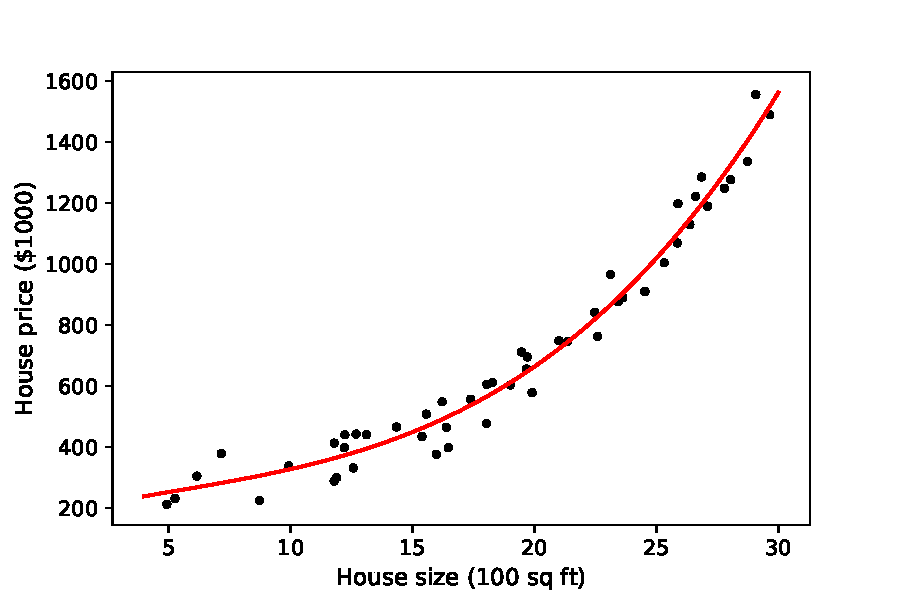
\includegraphics[scale=0.7]{images/lin_reg/poly-data.pdf}
\caption{Non-linear relationship between house price and size. Code used to generate this plot can be found \href{https://github.com/siavashaslanbeigi/ml_notes_supp/blob/master/lin_reg/poly.ipynb}{\color{blue} here}}.
\label{linreg-fig:poly-data}
\end{figure}


\appendix
% Linear Algebra =======================================
\section{Linear Algebra}
Here we present definitions and proofs of most linear algebra results used in the notes.
\begin{definition}
The conjugate transpose $A^*$ of an $m\times n$ complex matrix $A$ is an matrix $n \times m$ given by $A^*_{ij}=\overline{A_{ji}}$. In other words, first we transpose $A$ and then take the complex conjugate of every entry, as such:
\begin{equation}
    A =
    \begin{pmatrix}
        1 & 1+i & 2i \\
        3+2i & 2 & 5 \\
    \end{pmatrix},
    \qquad
    A^* =
    \begin{pmatrix}
        1 & 3-2i \\
        1-i & 2 \\
        -2i & 5 \\
    \end{pmatrix}.
\end{equation}
\end{definition}

\begin{definition}
A square complex matrix $A$ is called Hermitian matrix if it is equal to its conjugate transpose $A=A^*$. The following is an example:
\begin{equation}
    A =
    \begin{pmatrix}
        1 & 1+i \\
        1-i & 1 \\
    \end{pmatrix}.
\end{equation}
When $A$ is real, this is equivalent to saying $A$ is symmetric.
\end{definition}

\begin{theorem}
Eigenvalues of a Hermitian matrix are real.
\end{theorem}
 
\begin{proof}
Let $A$ be a Hermitian matrix and consider its eigenvalues and eigenvectors:
\begin{equation}
    Av_n=\lambda_nv_n.
\end{equation}
Applying $v_n^*$ to both sides:
\begin{equation}
    \lambda_n |v_n|^2 = v_n^*Av_n = v_n^*A^*v_n = (Av_n)^*v_n = (\lambda_nv_n)^*v_n = \overline{\lambda_n}|v_n|^2
    \label{appendix-eq:eig}
\end{equation}
where $|v_n|^2=v_n^*v_n>0$. Therefore, $\lambda_n=\overline{\lambda_n}$, which means $\lambda_n$ is real.
\end{proof}

\begin{theorem}
Eigenvectors of a Hermitian matrix $A$ with different eigenvalues are orthogonal, i.e.
\begin{equation}
    \lambda_n\ne\lambda_m \to v_n^*v_m=0.
\end{equation}
\end{theorem}

\begin{proof}
\begin{equation}
    \lambda_mv_n^*v_m = v_n^*(\lambda_mv_m) = v_n^*Av_m = v_n^*A^*v_m = (Av_n)^*v_m = \lambda_nv_n^*v_m,
\end{equation}
where the last one uses the fact that $\lambda_n$ is real. Thus, we've shown $(\lambda_m - \lambda_n)v_n^*v_m = 0$, and since we're assuming $\lambda_n\ne\lambda_m$, it follows that $v_n^*v_m=0$.
\end{proof}


\end{document}